The UR5 co-bot will be able to play a game of checkers against a human opponent. In order for the robot to do this, the robot arm will need a gripper and a camera. The gripper will be needed to pick up checker pieces. This gripper could be magnetic or a suction cup. In the case of a magnetic gripper, the checker pieces themselves will need to also be magnetic. The robot arm will also need to be paired with a camera in order to see and detect the checkerboard and its pieces. This is so the robot arm can determine the current state of the game, and determine the next optimal move for a piece to take. The computer will communicate with the robot arm and issue commands for it to make a particular move. Shown in Figure 1 is a high-level view of the implementation.

\begin{figure}[h!]
    \centering
    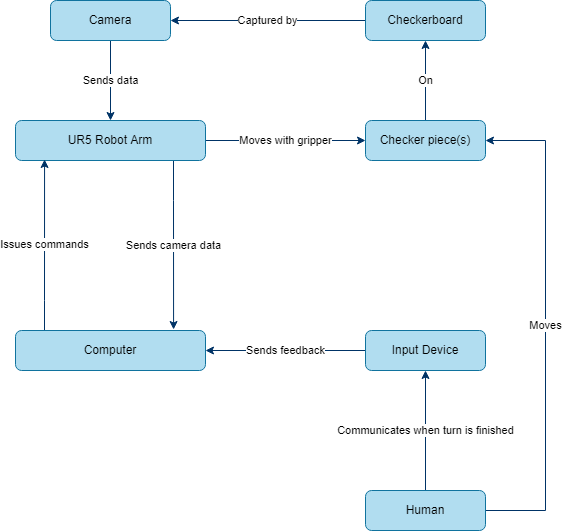
\includegraphics[width=0.8\textwidth]{images/system-overview.drawio.png}
    \caption{System Overview}
\end{figure}

As is illustrated in Figure 1, when the human player makes a move, the human must use some input device to communicate to the computer that they have completed their turn and it is now the UR5's turn to make a move. This input device could be a simple external button, or the computer keyboard. The computer is responsible for being the interface that communicates with the robot arm on what move it should make, how it should move, and any other commands needed to control it. Additionally, the computer will process the data received from the camera on the robot arm utilizing computer vision.

% Explain, at a high level, how you will implement a solution to the problem. Include a diagram of major components to the system (not a full architectural design, but a high level overview of the major system components and how a user or external system might interface). Avoid specific implementation details (operating system, programming languages, etc.). This section should occupy at least 1 full page.